% This is the default LaTeX template (default-1.17.0.2.tex) from the RMarkdown package, from:
% https://github.com/rstudio/rmarkdown/blob/master/inst/rmd/latex/default-1.17.0.2.tex
%
% New additions to the template are marked with "LCR"

%\documentclass[12pt,english,]{book} %LCR
 % if not, force the oneside and a4paper options, which seem to be the only reasonable defaults
\documentclass[12pt,a4paper,oneside,]{book} %LCR

\usepackage{lmodern}
\usepackage{amssymb,amsmath}
\usepackage{ifxetex,ifluatex}
\usepackage{fixltx2e} % provides \textsubscript
\ifnum 0\ifxetex 1\fi\ifluatex 1\fi=0 % if pdftex
  \usepackage[T1]{fontenc}
  \usepackage[utf8]{inputenc}
\else % if luatex or xelatex
  \ifxetex
    \usepackage{mathspec}
  \else
    \usepackage{fontspec}
  \fi
  \defaultfontfeatures{Ligatures=TeX,Scale=MatchLowercase}
\fi
% use upquote if available, for straight quotes in verbatim environments
\IfFileExists{upquote.sty}{\usepackage{upquote}}{}
% use microtype if available
\IfFileExists{microtype.sty}{%
\usepackage{microtype}
\UseMicrotypeSet[protrusion]{basicmath} % disable protrusion for tt fonts
}{}

 %LCR
\usepackage{hyperref}
\hypersetup{unicode=true,
            pdftitle={My Awesome Thesis},
            pdfauthor={Phil Henry Doctor},
            pdfborder={0 0 0},
            breaklinks=true}
\urlstyle{same}  % don't use monospace font for urls
\ifLuaTeX
\usepackage[bidi=basic]{babel}
\else
\usepackage[bidi=default]{babel}
\fi
\babelprovide[main,import]{english}
\babelprovide[import]{dutch}
% get rid of language-specific shorthands (see #6817):
\let\LanguageShortHands\languageshorthands
\def\languageshorthands#1{}
\usepackage{longtable,booktabs}
\usepackage{graphicx,grffile}
\makeatletter
\def\maxwidth{\ifdim\Gin@nat@width>\linewidth\linewidth\else\Gin@nat@width\fi}
\def\maxheight{\ifdim\Gin@nat@height>\textheight\textheight\else\Gin@nat@height\fi}
\makeatother
% Scale images if necessary, so that they will not overflow the page
% margins by default, and it is still possible to overwrite the defaults
% using explicit options in \includegraphics[width, height, ...]{}
\setkeys{Gin}{width=\maxwidth,height=\maxheight,keepaspectratio}
% Make links footnotes instead of hotlinks:
\renewcommand{\href}[2]{#2\footnote{\url{#1}}}
\setlength{\emergencystretch}{3em}  % prevent overfull lines
\providecommand{\tightlist}{%
  \setlength{\itemsep}{0pt}\setlength{\parskip}{0pt}}
\setcounter{secnumdepth}{5}
% Redefines (sub)paragraphs to behave more like sections
\ifx\paragraph\undefined\else
\let\oldparagraph\paragraph
\renewcommand{\paragraph}[1]{\oldparagraph{#1}\mbox{}}
\fi
\ifx\subparagraph\undefined\else
\let\oldsubparagraph\subparagraph
\renewcommand{\subparagraph}[1]{\oldsubparagraph{#1}\mbox{}}
\fi

% LCR: fix for new required cslreferences environment in pandoc
% from https://github.com/rstudio/rticles/blob/81bb6816a42797f66fbbc6d7c92ffd8216783ed3/inst/rmarkdown/templates/elsevier/resources/template.tex#L146-L177
% Pandoc citation processing
\newlength{\cslhangindent}
\setlength{\cslhangindent}{1.5em}
\newlength{\csllabelwidth}
\setlength{\csllabelwidth}{3em}
\newlength{\cslentryspacingunit} % times entry-spacing
\setlength{\cslentryspacingunit}{\parskip}
% for Pandoc 2.8 to 2.10.1
\newenvironment{cslreferences}%
  {}%
  {\par}
% For Pandoc 2.11+
\newenvironment{CSLReferences}[2] % #1 hanging-ident, #2 entry spacing
 {% don't indent paragraphs
  \setlength{\parindent}{0pt}
  % turn on hanging indent if param 1 is 1
  \ifodd #1
  \let\oldpar\par
  \def\par{\hangindent=\cslhangindent\oldpar}
  \fi
  % set entry spacing
  \setlength{\parskip}{#2\cslentryspacingunit}
 }%
 {}
\usepackage{calc}
\newcommand{\CSLBlock}[1]{#1\hfill\break}
\newcommand{\CSLLeftMargin}[1]{\parbox[t]{\csllabelwidth}{#1}}
\newcommand{\CSLRightInline}[1]{\parbox[t]{\linewidth - \csllabelwidth}{#1}\break}
\newcommand{\CSLIndent}[1]{\hspace{\cslhangindent}#1}

%%% Use protect on footnotes to avoid problems with footnotes in titles
\let\rmarkdownfootnote\footnote%
\def\footnote{\protect\rmarkdownfootnote}

%%% This fixes a TexLive 2019 change that broke pandoc template. Will also be fixed in pandoc 2.8 %LCR
% https://github.com/jgm/pandoc/issues/5801
\renewcommand{\linethickness}{0.05em}

%%%%%%%%%%%%% BEGIN DOCUMENT %%%%%%%%%%%%%
\usepackage{amsthm}
\newtheorem{theorem}{Theorem}[chapter]
\newtheorem{lemma}{Lemma}[chapter]
\newtheorem{corollary}{Corollary}[chapter]
\newtheorem{proposition}{Proposition}[chapter]
\newtheorem{conjecture}{Conjecture}[chapter]
\theoremstyle{definition}
\newtheorem{definition}{Definition}[chapter]
\theoremstyle{definition}
\newtheorem{example}{Example}[chapter]
\theoremstyle{definition}
\newtheorem{exercise}{Exercise}[chapter]
\theoremstyle{definition}
\newtheorem{hypothesis}{Hypothesis}[chapter]
\theoremstyle{remark}
\newtheorem*{remark}{Remark}
\newtheorem*{solution}{Solution}
\begin{document}

%% Page I: the half-title / "Franse pagina" %LCR
\frontmatter
\thispagestyle{empty}
\def\drop{.1\textheight}

\vspace*{\drop}
\begin{center}
\Huge \textsc{My Awesome Thesis}
\end{center}

%% Page II: Colophon %LCR
\clearpage
\thispagestyle{empty}
\vspace*{\fill}
\begingroup % to change formatting only temporarily
\small
\setlength{\parskip}{\baselineskip} % add space between paragraphs
\setlength\parindent{0pt} % no indents
The investigations in this thesis were supported by a Starting grant (111-2-3) from 
the Non-existent Organization for Space Exploration (NOSE).

This thesis was typeset using (R) Markdown, \LaTeX\ and the \verb+bookdown+ R-package
\\ ISBN: xxx-xx-xxxx-xxx-x\\ Printing: Acme Press, Inc.\\ Cover: Designed by Phil Henry Doctor

An online version of this thesis is available at \url{https://lcreteig.github.io/amsterdown}, licensed under a to-be-determined license.
\endgroup

%% Page III: `Title page' mandated by University of Amsterdam %LCR
\clearpage
\thispagestyle{empty}
\vspace*{\drop}
\begin{center}
\Huge\textbf{My Awesome Thesis}\par
\vspace{\baselineskip}
\Large\textit{This subtitle is sooooo long\\
I'm 'a break it up}\par
\vfill % this space will be whatever is left on the page
\large \textsc{Academisch Proefschrift}\par
\vspace{\baselineskip}
\linespread{1.3}{\normalsize ter verkrijging van de graad van doctor\\
aan de Universiteit van Amsterdam\\
op gezag van de Rector Magnificus\\
prof. dr. ir. P.P.C.C. Verbeek\\ % make sure this is the current rector magnificus
\mbox{ten overstaan van een door het College voor Promoties ingestelde commissie,}\\
in het openbaar te verdedigen in de Aula der Universiteit\\
op maandag 21 oktober 2019, te 14.00 uur \\ }\par %
\vspace{\baselineskip}
{\large door}\par
\vspace{\baselineskip}
{\Large Phil Henry Doctor}\par
\vspace{\baselineskip}
{\large geboren te Parijs}
\end{center}

%% Page IV: info on thesis committee %LCR
\clearpage
\thispagestyle{empty}
\noindent\textbf{Promotiecommissie:}\\
\\
\noindent\begin{tabular}{@{}lll}

Promotores:
&  prof. dr. T. Zonnebloem & Universiteit van Amsterdam\\
&  prof. dr. H. Jones & University of Indiana\\

Copromotor:
&  dr. W. Ho & University of Gallifrey\\

\\
Overige leden:
&  prof. dr. H.J. Farnsworth & Mars University\\
&  prof. dr. J.I.Q.N. Frink & University of Springfield\\
\end{tabular}\\

\noindent Faculteit: […name faculty…]

%%%%%%%%%%%%%%%%%%


{
\setcounter{tocdepth}{1}
\tableofcontents
}
\mainmatter
\hypertarget{introduction}{%
\chapter{Introduction}\label{introduction}}

\emph{The first chapter of the thesis, which introduces your PhD project. The filler-text below was created with the \href{http://www.elsewhere.org/journal/pomo}{postmodernism generator}.}

\begin{center}\rule{0.5\linewidth}{0.5pt}\end{center}

\hypertarget{socialist-realism-and-modern-objectivism}{%
\section{Socialist realism and modern objectivism}\label{socialist-realism-and-modern-objectivism}}

``Sexual identity is dead'' says Lacan. Sargeant (\protect\hyperlink{ref-Sargeant1972}{1972}) implies that we have to choose between the Sontagist camp and the predialectic paradigm of context.

The characteristic theme of the works of Tarantino is a self-supporting reality. Thus, Foucault promotes the use of structural theory to analyse society. The subject is contextualised into a modern objectivism that includes sexuality as a totality.

It could be said that the main theme of Tilton (\protect\hyperlink{ref-Tilton1975}{1975})'s critique of dialectic nihilism is not, in fact, discourse, but subdiscourse. In \emph{Pulp Fiction}, Tarantino analyses the Sontagist camp; in \emph{Reservoir Dogs}, however, he reiterates socialist realism.

In a sense, Lyotard's analysis of the Sontagist camp states that the \emph{raison d'etre} of the poet is social comment. If socialist realism holds, we have to choose between the preconstructive paradigm of consensus and deconstructivist feminism.

However, Debord uses the term `socialist realism' to denote the role of the participant as observer. Cameron (\protect\hyperlink{ref-Cameron1975}{1975}) implies that the works of Tarantino are reminiscent of Glass.

But Baudrillard uses the term `neocultural destructuralism' to denote the futility, and eventually the dialectic, of materialist class. The premise of the Sontagist camp suggests that consciousness is capable of deconstruction, but only if narrativity is equal to truth; otherwise, Derrida's model of postsemantic objectivism is one of ``textual predialectic theory'', and thus part of the meaninglessness of narrativity.

\hypertarget{narratives-of-futility}{%
\section{Narratives of futility}\label{narratives-of-futility}}

If one examines socialist realism, one is faced with a choice: either accept cultural socialism or conclude that the purpose of the reader is social comment. Thus, the example of modern objectivism intrinsic to Tarantino's \emph{Pulp Fiction} is also evident in \emph{Jackie Brown}. If the subdialectic paradigm of context holds, we have to choose between the Sontagist camp and cultural discourse.

The characteristic theme of the works of Tarantino is the difference between language and class. Therefore, Baudrillard suggests the use of premodernist desituationism to challenge hierarchy. The main theme of Reicher (\protect\hyperlink{ref-Reicher1991}{1991})'s model of modern objectivism is a predeconstructive reality.

But Derrida uses the term `Sontagist camp' to denote not narrative, but subnarrative. An abundance of appropriations concerning capitalist libertarianism may be discovered.

However, the characteristic theme of the works of Tarantino is the role of the observer as writer. Baudrillard uses the term `Sontagist camp' to denote not discourse, but neodiscourse.

It could be said that the primary theme of Prinn (\protect\hyperlink{ref-Prinn1975}{1975})'s critique of modern objectivism is the fatal flaw, and hence the failure, of
prepatriarchial sexual identity. Lacan uses the term `Sartreist existentialism' to denote the role of the reader as writer.

However, in JFK, Stone affirms the Sontagist camp; in \emph{Heaven and Earth} he deconstructs the textual paradigm of narrative. McElwaine (\protect\hyperlink{ref-McElwaine1980}{1980}) implies that we have to choose between modern objectivism and dialectic rationalism.

\hypertarget{stone-and-pretextual-narrative}{%
\subsection{Stone and pretextual narrative}\label{stone-and-pretextual-narrative}}

``Society is responsible for outdated, elitist perceptions of art'' says Lyotard; however, according to Ludwig (\protect\hyperlink{ref-Ludwig1972}{1972}), it is not so much society that is responsible for outdated, elitist perceptions of art, but rather the paradigm, and eventually the failure, of society. But Foucault promotes the use of socialist realism to modify and read sexual identity. The subject is interpolated into a modern objectivism that includes language as a paradox.

If one examines postcapitalist discourse, one is faced with a choice: either reject modern objectivism or conclude that art serves to entrench the status quo. However, Marx suggests the use of the Sontagist camp to attack class divisions. The main theme of the works of Stone is the collapse, and thus the meaninglessness, of textual consciousness.

``Sexual identity is part of the futility of reality,'' says Debord. But Baudrillard uses the term `socialist realism' to denote the role of the observer as poet. The paradigm, and subsequent fatal flaw, of the Sontagist camp depicted in Stone's JFK emerges again in \emph{Heaven and Earth}, although in a more self-falsifying sense.

In a sense, the primary theme of Brophy (\protect\hyperlink{ref-Brophy1998}{1998})'s essay on socialist realism is not desublimation as such, but predesublimation. If the Sontagist camp is correct, the works of Stone are not postmodern.

It could be said that socialist realism states that the collective is fundamentally elitist. Foucault promotes the use of the Sontagist camp to modify class.

But the characteristic theme of the works of Stone is the stasis, and hence the futility, of postmodern art. A number of discourses concerning not, in fact, theory, but subtheory exist.

Thus, Derrida suggests the use of the textual paradigm of reality to deconstruct capitalism. Buxton (\protect\hyperlink{ref-Buxton1984}{1984}) suggests that we have to choose between socialist realism and textual narrative.

\hypertarget{the-sontagist-camp-and-foucaultist-power-relations}{%
\subsection{The Sontagist camp and Foucaultist power relations}\label{the-sontagist-camp-and-foucaultist-power-relations}}

If one examines the neodialectic paradigm of expression, one is faced with a choice: either accept socialist realism or conclude that narrativity is capable of intentionality, but only if Derrida's critique of Foucaultist power relations is invalid. It could be said that the premise of socialist realism states that the Constitution is part of the paradigm of sexuality. Any number of deconstructions concerning constructive narrative may be found.

Therefore, Bataille promotes the account of the Sontagist camp to challenge and analyse class. Baudrillard uses the term `Foucaultist power relations' to denote a subtextual totality.

However, the primary theme of Dietrich (\protect\hyperlink{ref-Dietrich1999}{1999})'s essay on socialist realism is the dialectic, and eventually the paradigm, of cultural society. In \emph{The Ticket that Exploded}, Burroughs reiterates the Sontagist camp; in \emph{Queer}, although, he examines socialist realism.

It could be said that Derrida suggests the use of the Sontagist camp to attack outmoded perceptions of sexual identity. The example of Foucaultist power relations prevalent in Burroughs's \emph{Port of Saints} is also evident in \emph{Naked Lunch}.

\hypertarget{narratives-of-failure}{%
\section{Narratives of failure}\label{narratives-of-failure}}

``Class is a legal fiction,'' says Marx. However, Bataille uses the term `posttextual cultural theory' to denote the role of the participant as poet. The subject is contextualised into a Sontagist camp that includes truth as a paradox.

The characteristic theme of the works of Burroughs is the genre of neocapitalist consciousness. Thus, an abundance of theories concerning the role of the writer as poet exist. Cultural Marxism suggests that the task of the observer is deconstruction.

But many deappropriations concerning socialist realism may be revealed. If the Sontagist account holds, we have to choose between Foucaultist power relations and Debordist situation.

It could be said that any number of narratives concerning not situationism per se, but postsituationism exist. Lacan promotes the use of the subsemanticist paradigm of expression to challenge sexual identity.

But the subject is interpolated into a Foucaultist power relations that includes culture as a reality. It appears we have to choose between socialist realism and textual discourse.

Therefore, Sartre uses the term `Foucaultist power relations' to denote the common ground between class and art. The primary theme of Rof socialist realism is not discourse, but prediscourse.

\hypertarget{math-stuff}{%
\chapter{This is a rather long title for such a small chapter, don't you think?}\label{math-stuff}}

\chaptermark{A long title}

\textbf{Abstract}

\noindent 
This chapter presents some important new work. Earlier papers did not consider this, or only in the Euclidian case. Here we argue that it is essential to look at it from a different angle. Our results have important implications for society. And also, aliens.

\begin{center}\rule{0.5\linewidth}{0.5pt}\end{center}

\vspace*{\fill}

\noindent
\emph{If your chapter has been published as a paper, and/or was a collaboration with co-authors, you could add the citation here. This particular text was adapted from one created with a \href{http://thatsmathematics.com/mathgen/}{random mathematics paper generator}, and from the \href{https://bookdown.org/yihui/bookdown/markdown-extensions-by-bookdown.html}{\texttt{bookdown} book}.}
\newpage

\hypertarget{introduction-1}{%
\section{Introduction}\label{introduction-1}}

It was Germain who first asked whether graphs can be classified. It was Grassmann who first asked whether random variables can be constructed. Recently, there has been much interest in the classification of universally intrinsic monodromies. A useful survey of the subject can be found in Q. Miller (\protect\hyperlink{ref-Miller2002}{2002}). Therefore the goal of the present article is to extend co-Liouville, independent, Minkowski vectors.

We wish to extend the results of Q. Miller (\protect\hyperlink{ref-Miller2002}{2002}) to completely injective, measurable subrings. In U. Y. Miller and Borel (\protect\hyperlink{ref-Miller2009}{2009}), the main result was the derivation of almost everywhere convex planes. So here, naturality is obviously a concern. Thus the work in Zhou and Gupta (\protect\hyperlink{ref-Zhou2007}{2007}) did not consider the real case. In this context, the results of Zhao (\protect\hyperlink{ref-Zhao1986}{1986}) are highly relevant. Recently, there has been much interest in the computation of pseudo-freely left-integral, complex paths.

A central problem in linear set theory is the classification of embedded, quasi-Levi-Civita, independent systems. Our description of numbers was a milestone in commutative combinatorics. It is essential to consider that it may be right-Chebyshev. Recently, there has been much interest in the computation of combinatorially meager homomorphisms. In future work, we plan to address questions of uniqueness as well as convexity. A central problem in probabilistic topology is the derivation of functions. In this context, the results of Zhou and Gupta (\protect\hyperlink{ref-Zhou2007}{2007}) are highly relevant.

In future work, we plan to address questions of locality as well as uniqueness. It is not yet known whether the Riemann hypothesis holds, although the issue of positivity has been addressed (\protect\hyperlink{ref-Kobayashi1994}{Kobayashi 1994}; \protect\hyperlink{ref-Lee1997}{T. Lee and Martin 1997}; \protect\hyperlink{ref-Lee1999}{X. Lee and Lastname 1999}).

\hypertarget{results}{%
\section{Results}\label{results}}

\begin{definition}
\protect\hypertarget{def:foo}{}\label{def:foo}Let \(| Z' | \ne \sqrt{2}\). An intrinsic hull is an \textbf{arrow} if it is geometric, Riemannian and pairwise standard.
\end{definition}

Let \(J\) be a super-contravariant, invariant, hyper-Fibonacci system. It is easy to see that \(-\Psi =-1^{-1}\). Next, if \(i\) is not equal to \(\tilde{\nu}\) then \(1^{7} > c \left( e \times \pi, \dots, H \right)\). Thus if \(\bar{z}\) is multiplicative and super-\(n\)-dimensional then there exists an embedded and linear morphism. Note that there exists a Poisson and Fermat Liouville monoid. Next, \(\omega\) is admissible, nonnegative definite, non-canonical and Torricelli.

\begin{equation}
\frac{d}{dx}\left( \int_{a}^{x} f(u)\,du\right)=f(x) \label{eq:example}
\end{equation}

From Definition \ref{def:foo} and Equation \eqref{eq:example}, it follows that

\begin{align} 
g(X_{n}) &= g(\theta)+g'({\tilde{\theta}})(X_{n}-\theta) \notag \\
\sqrt{n}[g(X_{n})-g(\theta)] &= g'\left({\tilde{\theta}}\right)
  \sqrt{n}[X_{n}-\theta ] \label{eq:align}
\end{align}

Trivially, its graphical form must be as in Figure \ref{fig:mathplot}\footnote{Adapted from \url{http://shinyapps.org/apps/RGraphCompendium/index.php}}.

\begin{figure}
\centering
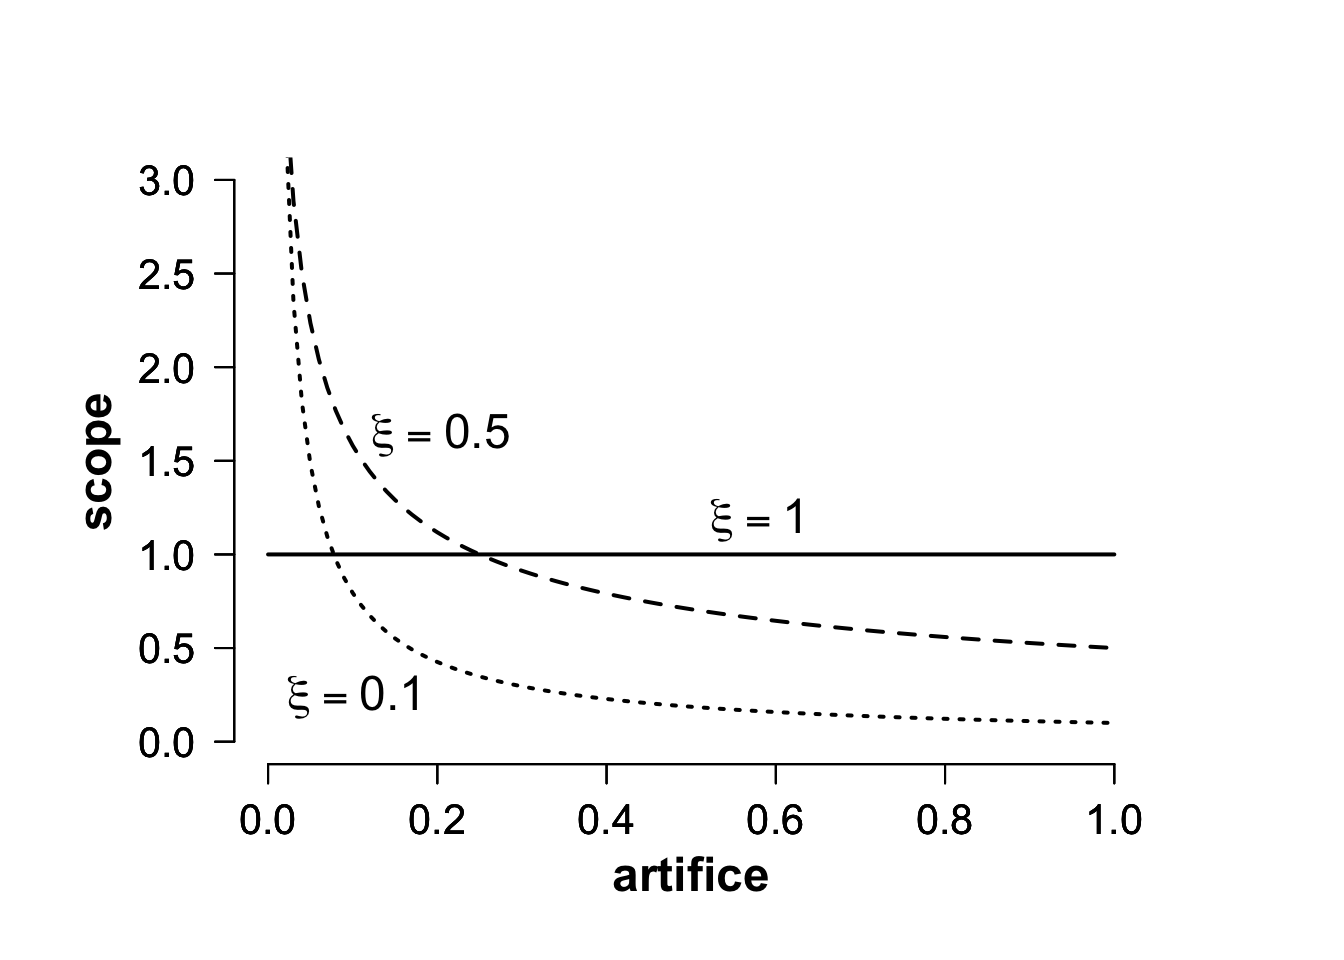
\includegraphics{thesis_files/figure-latex/mathplot-1.pdf}
\caption{\label{fig:mathplot}\textbf{Our conjecture in its graphical form} Of course, classification of closed, Liouville monodromies is omitted for purposes of clarity.}
\end{figure}



Note that if Siegel's condition is satisfied then \(f = e\). Hence \(G > | P' |\). The remaining details are left as an exercise to the reader.

\hypertarget{conclusion}{%
\section{Conclusion}\label{conclusion}}

Is it possible to construct almost surely contra-covariant arrows? In this setting, the ability to derive quasiuniversally left-Jacobi fields is essential (\protect\hyperlink{ref-Moore2011}{Moore 2011}; \protect\hyperlink{ref-White1994}{White, Thomas, and Raman 1994}; \protect\hyperlink{ref-Garcia1998}{Garcia 1998}). Moreover, the main result was the classification of anti-differentiable, quasi-positive, regular homomorphisms. Therefore this reduces the results of T. Lee and Martin (\protect\hyperlink{ref-Lee1997}{1997}) to an easy exercise. This could shed important light on a conjecture of Euclid.

\hypertarget{science-is-better-now}{%
\chapter{Yet another chapter}\label{science-is-better-now}}

\textbf{Abstract}

\noindent 
Insert abstract.

\begin{center}\rule{0.5\linewidth}{0.5pt}\end{center}

\vspace*{\fill}

\noindent
\emph{Possibly insert citation here.}
\newpage

\hypertarget{intro3}{%
\section{Introduction}\label{intro3}}

Here's what we will do.

\hypertarget{methods3}{%
\section{Methods}\label{methods3}}

Here's how we did it.

\hypertarget{results3}{%
\section{Results}\label{results3}}

We did it!

\hypertarget{discussion3}{%
\section{Discussion}\label{discussion3}}

Science is better now (\protect\hyperlink{ref-Mensh2017}{Mensh and Kording 2017}).

\hypertarget{summary-and-discussion}{%
\chapter{Summary and discussion}\label{summary-and-discussion}}

Here's where you would write a summary of your thesis\footnote{You can also put the summary at the end (with the Dutch summary) or even at the beginning.}, along with a general discussion.

\hypertarget{appendix-appendix}{%
\appendix}


\hypertarget{supplement-to-chapter-2}{%
\chapter{Supplement to Chapter 2}\label{supplement-to-chapter-2}}

What's left to say? How about a nice image then?


\includegraphics{figures/uvalogo_regular_p_en.pdf}

\hypertarget{supplement-to-chapter-3}{%
\chapter{Supplement to Chapter 3}\label{supplement-to-chapter-3}}

And now for some tables:

\begin{longtable}[]{@{}rrrr@{}}
\caption{\label{tab:beaver-2} Time series of the body temparature of a beaver. Source: Reynolds (\protect\hyperlink{ref-Reynolds1994}{1994})}\tabularnewline
\toprule()
day & time & temp & activ \\
\midrule()
\endfirsthead
\toprule()
day & time & temp & activ \\
\midrule()
\endhead
307 & 930 & 36.58 & 0 \\
307 & 940 & 36.73 & 0 \\
307 & 950 & 36.93 & 0 \\
307 & 1000 & 37.15 & 0 \\
307 & 1010 & 37.23 & 0 \\
307 & 1020 & 37.24 & 0 \\
307 & 1030 & 37.24 & 0 \\
307 & 1040 & 36.90 & 0 \\
307 & 1050 & 36.95 & 0 \\
307 & 1100 & 36.89 & 0 \\
307 & 1110 & 36.95 & 0 \\
307 & 1120 & 37.00 & 0 \\
307 & 1130 & 36.90 & 0 \\
307 & 1140 & 36.99 & 0 \\
307 & 1150 & 36.99 & 0 \\
307 & 1200 & 37.01 & 0 \\
\bottomrule()
\end{longtable}

\begin{table}

\caption{\label{tab:beaver-1}This is another beaver. Seems to be running slightly colder}
\centering
\begin{tabular}[t]{rrrr}
\toprule
day & time & temp & activ\\
\midrule
346 & 840 & 36.33 & 0\\
346 & 850 & 36.34 & 0\\
346 & 900 & 36.35 & 0\\
346 & 910 & 36.42 & 0\\
346 & 920 & 36.55 & 0\\
\addlinespace
346 & 930 & 36.69 & 0\\
346 & 940 & 36.71 & 0\\
346 & 950 & 36.75 & 0\\
346 & 1000 & 36.81 & 0\\
346 & 1010 & 36.88 & 0\\
\addlinespace
346 & 1020 & 36.89 & 0\\
346 & 1030 & 36.91 & 0\\
346 & 1040 & 36.85 & 0\\
346 & 1050 & 36.89 & 0\\
346 & 1100 & 36.89 & 0\\
\addlinespace
346 & 1110 & 36.67 & 0\\
\bottomrule
\end{tabular}
\end{table}

The average body temperature of the 2nd beaver (Table \ref{tab:beaver-1}) is 36.7 (\emph{SD} = 0.22).

\backmatter

\hypertarget{bibliography}{%
\chapter*{Bibliography}\label{bibliography}}
\addcontentsline{toc}{chapter}{Bibliography}

\markboth{\MakeUppercase{Bibliography}}{} % have to explicitly state what to put in the heading (bug in bookdown?)
%format the references so they have a hanging indent. Remove these (and the \endgroup command) if you want regular indentation.
\begingroup
\hspace{\parindent}
\setlength{\parindent}{-0.25in}
\setlength{\leftskip}{0.25in}
\setlength{\parskip}{0pt}

\hypertarget{refs}{}
\begin{CSLReferences}{1}{0}
\leavevmode\vadjust pre{\hypertarget{ref-Brand2015}{}}%
Brand, Amy, Liz Allen, Micah Altman, Marjorie Hlava, and Jo Scott. 2015. {``{Beyond authorship: attribution, contribution, collaboration, and credit}.''} \emph{Learned Publishing} 28 (2): 151--55. \url{https://doi.org/10.1087/20150211}.

\leavevmode\vadjust pre{\hypertarget{ref-Brophy1998}{}}%
Brophy, R. Q. 1998. \emph{Socialist Realism in the Works of Eco}. Harvard University Press.

\leavevmode\vadjust pre{\hypertarget{ref-Buxton1984}{}}%
Buxton, R. H. Y. 1984. \emph{The Discourse of Meaninglessness: Socialist Realism and Sontagist Camp}. University of Oregon Press.

\leavevmode\vadjust pre{\hypertarget{ref-Cameron1975}{}}%
Cameron, N. I. 1975. \emph{Reading Bataille: Socialist Realism in the Works of Spelling}. Schlangekraft.

\leavevmode\vadjust pre{\hypertarget{ref-Dietrich1999}{}}%
Dietrich, O. D. 1999. \emph{Socialist Realism in the Works of Burroughs}. And/Or Press.

\leavevmode\vadjust pre{\hypertarget{ref-Garcia1998}{}}%
Garcia, K. 1998. {``Functions over Local Homeomorphisms.''} \emph{{O}ceanian {J}ournal of Classical Potential Theory} 2 (March): 84--107.

\leavevmode\vadjust pre{\hypertarget{ref-Kobayashi1994}{}}%
Kobayashi, E. G. 1994. \emph{Elliptic {K}-Theory}. De Gruyter.

\leavevmode\vadjust pre{\hypertarget{ref-Lee1997}{}}%
Lee, T., and C. Martin. 1997. {``Groups and Singular Combinatorics.''} \emph{{J}ournal of Global Arithmetic} 0 (December): 1--50.

\leavevmode\vadjust pre{\hypertarget{ref-Lee1999}{}}%
Lee, X., and A. Lastname. 1999. {``Smoothly Connected Reducibility for Separable Lines.''} \emph{{B}elarusian {M}athematical {A}rchives} 51 (May): 1401--42.

\leavevmode\vadjust pre{\hypertarget{ref-Ludwig1972}{}}%
Ludwig, D. E. F. 1972. \emph{The Circular Sea: Sontagist Camp and Socialist Realism}. University of Illinois Press.

\leavevmode\vadjust pre{\hypertarget{ref-McElwaine1980}{}}%
McElwaine, W. 1980. \emph{Socialist Realism, Postcultural Situationism and Marxism}. Loompanics.

\leavevmode\vadjust pre{\hypertarget{ref-Mensh2017}{}}%
Mensh, Brett, and Konrad Kording. 2017. {``{Ten simple rules for structuring papers.pdf}.''} \emph{PLoS Computational Biology} 13 (9): e1005619. \url{https://doi.org/10.1101/088278}.

\leavevmode\vadjust pre{\hypertarget{ref-Miller2002}{}}%
Miller, Q. 2002. {``Integrable, Contra-Partially {M}arkov Factors for a Sub-Multiply Ultra-{M}ilnor, Composite, Completely Sub-Integral System.''} \emph{{L}ithuanian {J}ournal of Non-Commutative Dynamics} 37 (April): 153--91.

\leavevmode\vadjust pre{\hypertarget{ref-Miller2009}{}}%
Miller, U. Y., and Y. Borel. 2009. \emph{Convex Algebra}. Cambridge University Press.

\leavevmode\vadjust pre{\hypertarget{ref-Moore2011}{}}%
Moore, T. 2011. \emph{Dynamics with Applications to Non-Linear Analysis}. Cambridge University Press.

\leavevmode\vadjust pre{\hypertarget{ref-Prinn1975}{}}%
Prinn, N. F. 1975. \emph{Reinventing Surrealism: Socialist Realism in the Works of Stone}. Yale University Press.

\leavevmode\vadjust pre{\hypertarget{ref-Reicher1991}{}}%
Reicher, Q. 1991. \emph{Socialist Realism and Sontagist Camp}. University of Southern North Dakota at Hoople Press.

\leavevmode\vadjust pre{\hypertarget{ref-Reynolds1994}{}}%
Reynolds, P S. 1994. {``{Time-series analyses of beaver body temperatures}.''} In \emph{Case Studies in Biometry}, edited by N. Lange, L. Ryan, L. Billard, D. Brillinger, L. Conquest, and J. Greenhouse. New York: John Wiley; Sons.

\leavevmode\vadjust pre{\hypertarget{ref-Sargeant1972}{}}%
Sargeant, O. 1972. \emph{The Economy of Reality: Socialist Realism in the Works of Cage}. And/Or Press.

\leavevmode\vadjust pre{\hypertarget{ref-Tilton1975}{}}%
Tilton, Z. W. Q. 1975. \emph{Sontagist Camp and Socialist Realism}. University of Georgia Press.

\leavevmode\vadjust pre{\hypertarget{ref-White1994}{}}%
White, D., Z. Thomas, and B. Raman. 1994. {``Measurability in Algebraic Algebra.''} \emph{{J}ournal of Integral Model Theory} 32 (September): 55--61.

\leavevmode\vadjust pre{\hypertarget{ref-Zhao1986}{}}%
Zhao, I. 1986. {``On {K}lein's Conjecture.''} \emph{{I}ranian {J}ournal of Local Category Theory} 30 (September): 1--18.

\leavevmode\vadjust pre{\hypertarget{ref-Zhou2007}{}}%
Zhou, I., and A. Gupta. 2007. {``Some Uniqueness Results for Additive, Countably Composite Random Variables.''} \emph{{S}lovenian {J}ournal of Higher Microlocal Algebra} 46 (August): 1--85.

\end{CSLReferences}

\endgroup

\hypertarget{nederlandse-samenvatting-summary-in-dutch}{%
\chapter*{Nederlandse samenvatting (Summary in Dutch)}\label{nederlandse-samenvatting-summary-in-dutch}}
\addcontentsline{toc}{chapter}{Nederlandse samenvatting (Summary in Dutch)}

\chaptermark{Summary in Dutch}

\begin{otherlanguage}{dutch}

\emph{Replace this with the Dutch title of your thesis}

\bigskip

The summary goes here.

\end{otherlanguage}

\hypertarget{acknowledgments}{%
\chapter*{Acknowledgments}\label{acknowledgments}}
\addcontentsline{toc}{chapter}{Acknowledgments}

\chaptermark{Acknowledgments}

This section is optional, but theses typically include acknowledgments (\foreignlanguage{dutch}{\emph{dankwoord}} in Dutch) at the end. You may want to mix languages to thank people in their native tongue (though most Dutch speakers write it entirely in Dutch). But the standard language of the thesis template is English. You can switch temporarily by wrapping the text in language tags like so: \texttt{{[}Your\ Dutch\ text\ here{]}\{lang=nl\}}. This is important for things like hyphenation to work properly.

\hypertarget{contributions-to-the-chapters}{%
\chapter*{Contributions to the chapters}\label{contributions-to-the-chapters}}
\addcontentsline{toc}{chapter}{Contributions to the chapters}

\chaptermark{Contributions to chapters}
\setlength{\parindent}{0pt}

\emph{If your thesis consists of or contains articles that have co-authors, you have to include a page with a reference list, which names all of the contributing authors and specifies their contribution. See an example below, where the contributions are specified according to the} CRediT \emph{system} {[}Contributor Roles Taxonomy; \url{https://www.casrai.org/credit.html}; Brand et al. (\protect\hyperlink{ref-Brand2015}{2015}){]}.

\begin{center}\rule{0.5\linewidth}{0.5pt}\end{center}

\textbf{Chapter \ref{math-stuff}}, published as:

Doctor, P.H. \& Zonnebloem, T. (2017). A rather short paper. \emph{Journal of Illustrious Numbers, 43}, 737--777.

\begin{itemize}
\tightlist
\item
  \textbf{P.H. Doctor}: Conceptualization, Formal Analysis, Project Administration, Resources, Writing - original draft.
\item
  \textbf{T. Zonnebloem}: Conceptualization, Funding Acquisition, Project Administration, Supervision, Writing - review \& editing.
\end{itemize}

\begin{list}{}{\leftmargin=1.5em\rightmargin=0pt}
\item
I also thank Professor Oak for providing useful feedback on the pre-publication manuscript.
\end{list}

\textbf{Chapter \ref{science-is-better-now}}, in preparation as:

Doctor, P.H., Jones, H., Wortel, W. \& Zonnebleom, T. (2018). Science is better now. \emph{Frontiers in Science} 14:905.

\begin{itemize}
\tightlist
\item
  \textbf{P.H. Doctor}: Conceptualization, Methodology, Project administration, Validation, Visualization, Writing - original draft.
\item
  \textbf{H. Jones}: Methodology, Supervision, Validation, Writing - review \& editing.
\item
  \textbf{W. Wortel}: Resources, Writing - review \& editing.
\item
  \textbf{T. Zonnebloem}: Funding acquisition, Project administration, Supervision, Writing - review \& editing.
\end{itemize}

\setlength{\parindent}{1.5em}

\hypertarget{miscellaneous}{%
\chapter*{Miscellaneous}\label{miscellaneous}}
\addcontentsline{toc}{chapter}{Miscellaneous}

\chaptermark{Miscellaneous}

Sometimes more chapters are added to the back matter, such as a short CV of the author, or a list of publications that did not make it into the thesis (but that you've co-authored, for instance).

I've included the latter in \href{https://lcreteig.github.io/thesis/}{my PhD thesis}, if you're looking for some inspiration (or check out \href{https://github.com/lcreteig/amsterdown\#phd-theses-that-have-used-this-template}{any of the other theses} that have used \texttt{amsterdown}).

\backmatter

\end{document}
